\section{A steep learning curve: first leads in Primadona}

\subsection{Defeating the Gargantuan Boulder}
The expedition wasn't off to a great start. We spent one day bolting down the wrong valley, and it took another two pushing trips down the correct valley to get within sight of \passage{Primadona}. Tanguy and I had climbed up from the \passage{Kal}/\passage{Krn} path a couple of days before to verify this was the right way down, and the terrifying nature of the scree slope up again made us question the sanity of our Slovenian colleagues.

\begin{marginfigure}
\checkoddpage \ifoddpage \forcerectofloat \else \forceversofloat \fi
\centering
\frame{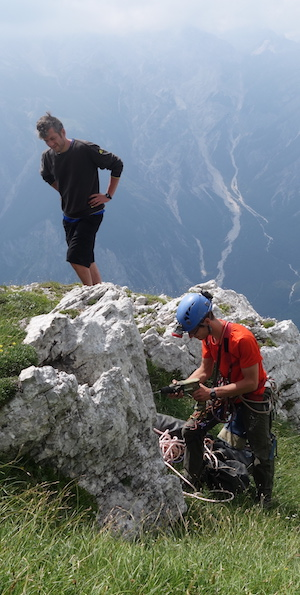
\includegraphics[width=\textwidth]{images/2016/jack-begin-2016/wrong-valley.jpg}}
\caption{Misguided by the presence of rusty spits in the rock, we started to rig the abseil two valleys too far south \pic{Rhys Tyers}}
\label{wrong valley}
\end{marginfigure}

Still, today we were in spitting distance, just a few short Y-hangs to go and then we'd be in. Tanguy and I recruited Miriam to help out, and we dropped down the increasingly familiar series of not really vertical pitches to the proper hangs. Miriam and I hung out on a ledge whilst Tanguy dropped down to place a few more bolts, and we relaxed, studying \passage{Krn} on the far side of the \passage{Tolminka} valley, which dropped away 1.4\,km below us.

\fullwidthbox{Finding the right valley}{
Gosh, what a day! Tanguy woke me early, luring me from my tent with the promise of porridge. Thus prepared for the day, I set off with Tanguy to \passage{Kal} and then on towards \passage{Krn}. You see, we had worked out that the 15 bolts Tanguy bolted yesterday were not leading to \passage{Primadona}. This involved reading some cryptic phrases in the hollow mountain, written in the passive voice with many question marks. It must have been written by an academic, I suspect Jarv. Regardless, we strode towards \passage{Krn}, looking right up the canyons to the plateau. We spotted the rock bridge and yesterday bolts, and it was clear that we were two valleys too far south. 
\name{Jack Hare}}

Soon we were down, and we encountered the huge snow slope in the entrance. Keen to demonstrate my winter hiking knowledge I spent some time kicking steps in, zig-zagging back and forth until we got to the bottom. The way on wasn't obvious, and I think Tanguy went through the crawl on the bottom left first. It was very tight the first time, but became increasingly wide over the next two weeks. We couldn't spot the stream Fratnik had warned us about, but tried to rig a tarp anyway in case it appeared during heavy rain. It never did, and tarp was soon derigged as a nuisance.

Tanguy handed me the drill and bolting kit, and I went out into the hading rift, roughly following the Slovenian rigging. I did a poor job on the first pitch, which was re-rerigged three or four times over the expo, but we were soon down. \bignote{The loose and dangerous nature of \passage{Primadona} was soon apparent and we spaced ourselves out}.

The next pitch has a tight pitch-head, and I just rigged next to the Slovenian bolts, a mixture of terrifying home made hangers, calcite encrusted krabs and rusted through-bolts. The rope left in situ wasn't much better - this was obviously a harsh environment for equipment. The bottom of the pitch was a very loose scree slope that didn't improve one bit during the expedition, despite Zdenko's best efforts on the next day.

The Slovenian's rope went round the corner on the left, but I thought a straight hang would be better, and I was sketched out by the thought of rigging a traverse that high up. As began to descend I looked up, and saw a huge boulder perched above me. It was unclear what was stopping it falling, about the size of a fridge and apparently leaning with its top on the far wall. As Miriam descended, I shouted up: `Hey Tanguy, interesting rock at the top of the pitch. Worth taking a look.' I was trying not to worry Miriam, and the tone of my voice must have communicated that to Tanguy because when he got to the bottom he muttered `Yes, we should do something about that.'

\begin{marginfigure}
\checkoddpage \ifoddpage \forcerectofloat \else \forceversofloat \fi
\centering
\frame{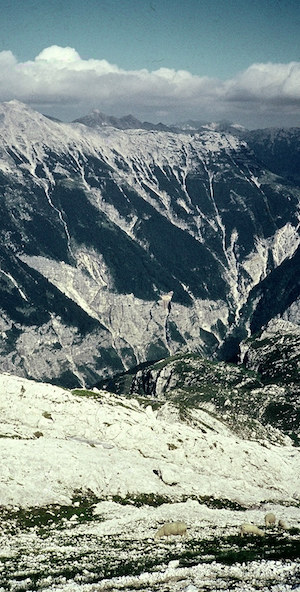
\includegraphics[width=\textwidth]{images/2016/jack-begin-2016/tolminski_kuk_157.jpg}}
\caption{A view of \protect\passage{Tolminski Migovec} from the \protect\passage{Krn} massif to the NW \pic{Anonymous}}
\label{view}
\end{marginfigure}

We got to the top of the next pitch head, a nice Y-hang into the chamber where the bear skeleton had been found, and found we were out of rope - the cave really eats it! Tanguy and Miriam ascended first, and we quickly realised the scree was so loose that it's necessary for those above to get clear off the floor before the next person ascends.

With Tanguy and Miriam safely out of the way, I ascended to the top of the first rebelay and clipped into the traverse. I derigged the rope below to get it out of the way, and clipped my hand jammer into the rope. Climbing up above the last bolt and onto the ledge with the boulder on, I realised quite how terrifying the situation was. This huge rock was balanced on just two points of rock - one on the ledge by my feet, and one on the far wall. I reached out with a toe and gently tapped it. Whomp, whomp, whomp - it wobbled back and forth with ease. 

Preparing myself mentally and physically, I shouted up to Tanguy that I was about to remove the rock. With more force than was strictly necessary I reached out and gave it a firm kick. It immediately plummeted down, smashing into the walls as it went and creating a huge amount of noise. As the dust settled and my hearing returned I found I was screaming `I'm okay! I'm okay!' over and over again, probably to reassure myself. Tanguy seemed bemused and shouted back down to me. I rerigged and rejoined them at the top - Miriam especially was quite shocked at the noise and the carnage, and I think we all learned something about how loose and dangerous \passage{Primadona} was.

Why didn't we remove the rock before descending? Writing this, I'm not sure. I'd like to think there's a detail I missed that meant the others had to come down first, but it seems careless. Still, the first two pitches were now rebolted, and the way deeper into the cave was clear.

\begin{marginfigure}
\checkoddpage \ifoddpage \forcerectofloat \else \forceversofloat \fi
\centering
\frame{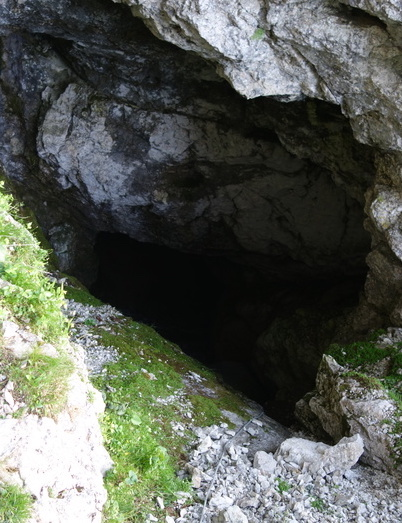
\includegraphics[width=\textwidth]{images/2016/jack-begin-2016/prima-ent.jpg}}
\caption{A gaping hole on the side of the cliff, some 120m below the Plateau entrance, the twin entrances of Primadona  \pic{Rhys Tyers}}
\label{prima entrance}
\end{marginfigure}
\subsection{Bolting the Superhighway}
The day started well. We had 200 metres of rope up the mountain thanks to Tanguy's heroic carry, and Zdenko and Izi had arrived the night before, keen to take us deeper into \passage{Primadona} than we'd been before. Kenneth was keen to do some bolting, and a lot of the Slovenian rigging we'd encountered had decayed with time and needed replacing. The obvious solution - we would go in first, and the other parties would catch us up, allowing them to benefit from the new rigging.

I kindly offered Kenneth the opportunity to carry down all of the rope, but after realising it would have to be on his back instead of dangling below (too much loose rock) he kindly offered the opportunity to me instead. Grumbling, stumbling and sweating I picked my way down the cliff face, kicking off very few rocks. We quickly passed the first three pitches that had been rigged the day before, and paused to examine the pulverised remains of the massive boulder that had been gardened the previous day.

\begin{marginfigure}
\checkoddpage \ifoddpage \forcerectofloat \else \forceversofloat \fi
\centering
 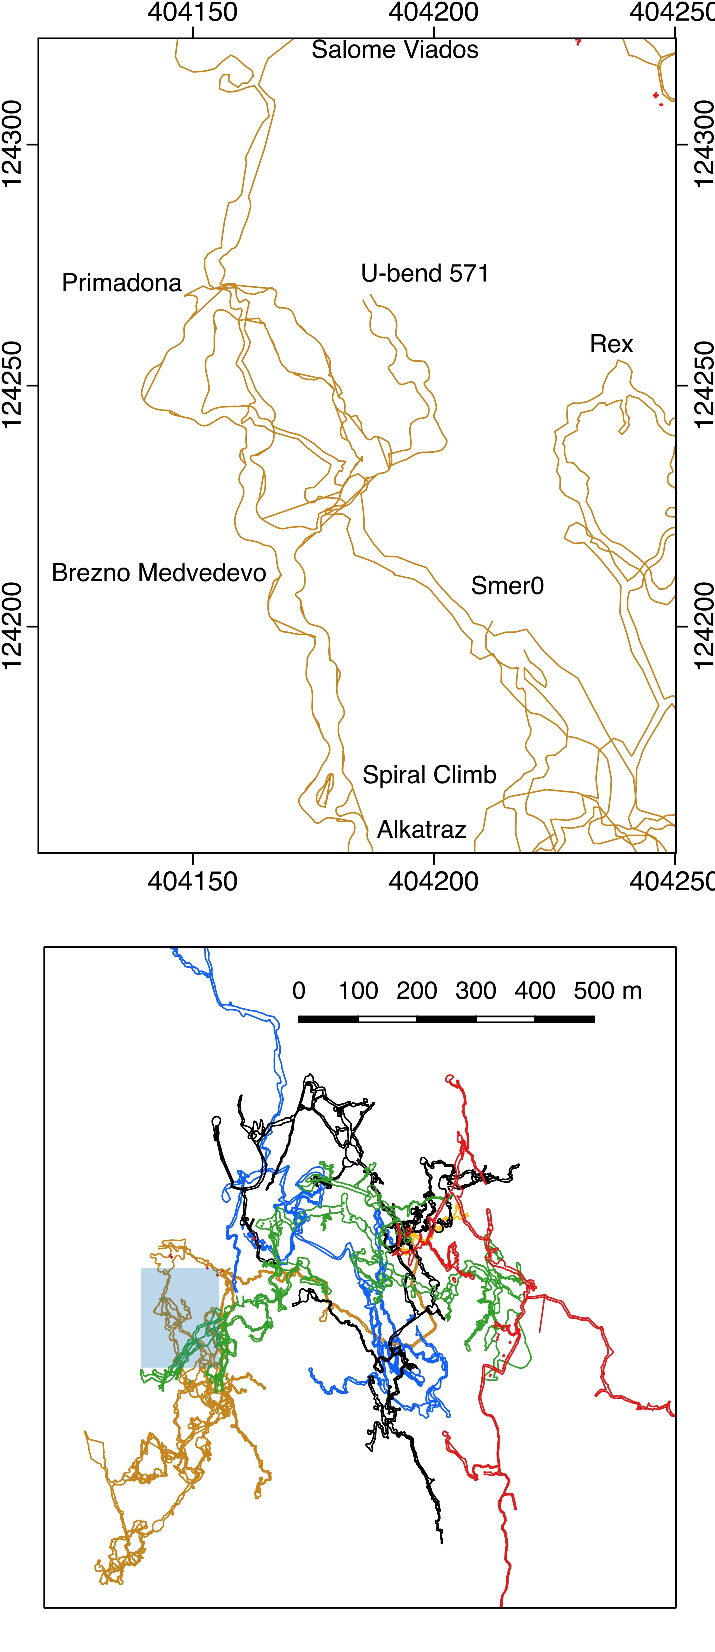
\includegraphics[width=\linewidth]{images/little_insets/ent_prim_inset.pdf}
 \caption{Plan view of the entrance series to \protect\passage{Primadona}. Slovenian National Grid ESPG 3794}
 \label{prim ent inset}
\end{marginfigure}

The pitch into \passage{Bear Pitch} (where the skeleton of a young bear had been found) was next to be rebolted. Kenneth set to work, tapping rocks and thinking about positions. I free climbed around a bit, and then settled down and started giving him advice. It was a nice clean Y-hang (in my opinion, the highest and most beautiful rigging possible) and Kenneth was quick and efficient. Before we could go any further, Zdenko, with Will S and Rhys in tow, passed us.

The next pitch I think is nameless - it starts with a traverse in a rift, and drops into a large cavern and the wall slopes outwards at the bottom. No rebelay necessary and we were soon down. \bignote{On the previous day's trip we had mostly emulated the Slovenian rigging, but today we began to add our own twists to it}. At the bottom a rift opened up in the centre of the cavern, with wide ledges on either side. The Slovenian rigging was very expedition style - the rope dropped down immediately into the rift with a tight and unpleasant rebelay which we had the pleasure of watching Izi's group do. Izi made it easy by not bothering to really clip into anything, but the rest struggled. Watching this, Kenneth and I decided we had to do a better job.

Kenneth traversed out along the rift until the walls were close enough to put in a nice Y-hang. With two little ledges on either side and a good clean drop it was a beautiful Y-hang, and after some encouragement everyone told me so that evening. At the bottom was a free climb (later with a rope added) and then the \passage{Spiral Climb}, with an anti-clockwise spiral down. It took a little time to find the way on (both Zdenko and Izi's team had been here already, so we knew there had to be one) but eventually it was found in a low bedding plane rift. It was drippy and cold down there, so I left Kenneth, confident that by now he knew how to rig.

\begin{pagefigure}
    \checkoddpage \ifoddpage \forcerectofloat \else \forceversofloat \fi
    \centering
    \begin{subfigure}[t]{0.681\textwidth}
        \centering
        \frame{\includegraphics[width=\linewidth]{"images/2016/jack-begin-2016/prima-fault".jpg}}
        \caption{} \label{Traverse over buckwheat}
    \end{subfigure}
        \hfill
    \begin{subfigure}[t]{0.303\textwidth}
        \centering
        \frame{\includegraphics[width=\linewidth]{"images/2016/jack-begin-2016/prima-beautiful".jpg}}
         \caption{}\label{passage in Deja VU}
    \end{subfigure}
    \vspace{0cm}

    \begin{subfigure}[t]{0.397\textwidth}
        \centering
        \frame{\includegraphics[width=\linewidth]{"images/2016/jack-begin-2016/prima-entrance-series".jpg}}
        \caption{} \label{Dejavu}
    \end{subfigure}
        \hfill
    \begin{subfigure}[t]{0.593\textwidth}
        \centering   
        \frame{\includegraphics[width=\linewidth]{"images/2016/jack-begin-2016/prima-bear".jpg}}
        \caption{} \label{Dejavu}
    \end{subfigure}

    \caption{
        \textit{(a)} The head of the entrance pitch in \protect\passage{Primadona} formed along a well-defined fault-plane
        \textit{(b)} The beautiful Y-hang pitch in the entrance series with Larry Jiyy Jiang at the take-off
        \textit{(c)} One of the larger entrance series pitches cuts across a prominent geological horizon
        \textit{(d)} Rebecca Diss at the top of the \protect\passage{Bear Pitch} where the 2000 era metal plates are still visible \pic{Rhys Tyers} }
\end{pagefigure}

Instead, I climbed back up the spiral to explore a lead that I'd noticed early. A rift came in from one side, extending vertically upwards for some way, with many ledges at various levels. I climbed up and traversed along the ledges until the rift became too tight, and then I climbed up another level. Repeating this a few times got me quite high above where I'd been, and the undisturbed nature of the mud convinced me that no one had bothered before - it was quite a lot of effort and not very promising. At the far end I found a tight crawl near the ceiling, with a good draft and the promise of a large chamber beyond. Not wanting to push my luck exploring without anyone else around, I turned back to find Kenneth.

He'd bolted most of the way down at this point, pausing to tackle a tricky rebelay (this was rebolted twice during the expedition - the final version is quite good). We could hear Zdenko, Rhys and Will below, and from our conversation we determined that they'd forgotten to bring a drill bit but really wanted to drill stuff. We promised them our spare and met them at the bottom. The water collected in sawn off plastic bottles was a welcome treat, and they seemed to have had a good day of exploration doing some slightly dodgy free climbs.

At this point we decided to turn round with Zdenko, whilst Will and Rhys bolted their dodgy free climb. It was a pleasure to ascend the rigging we'd just put in, and it felt like a quick ascent, at this point still new and exciting. I waited near the entrance to check if Zdenko was behind, and when he came into hearing range he said he couldn't hear Will or Rhys. He was too cold to go check on them, so I dropped the first few pitches until I could hear them and check they were fine - no problems, just a little delay.

Ascending in the sunset and looking over at \passage{Krn}, I couldn't help but think `gosh - what a day!'.


\subsection{The Rock}
\begin{marginfigure}
\checkoddpage \ifoddpage \forcerectofloat \else \forceversofloat \fi
\centering
 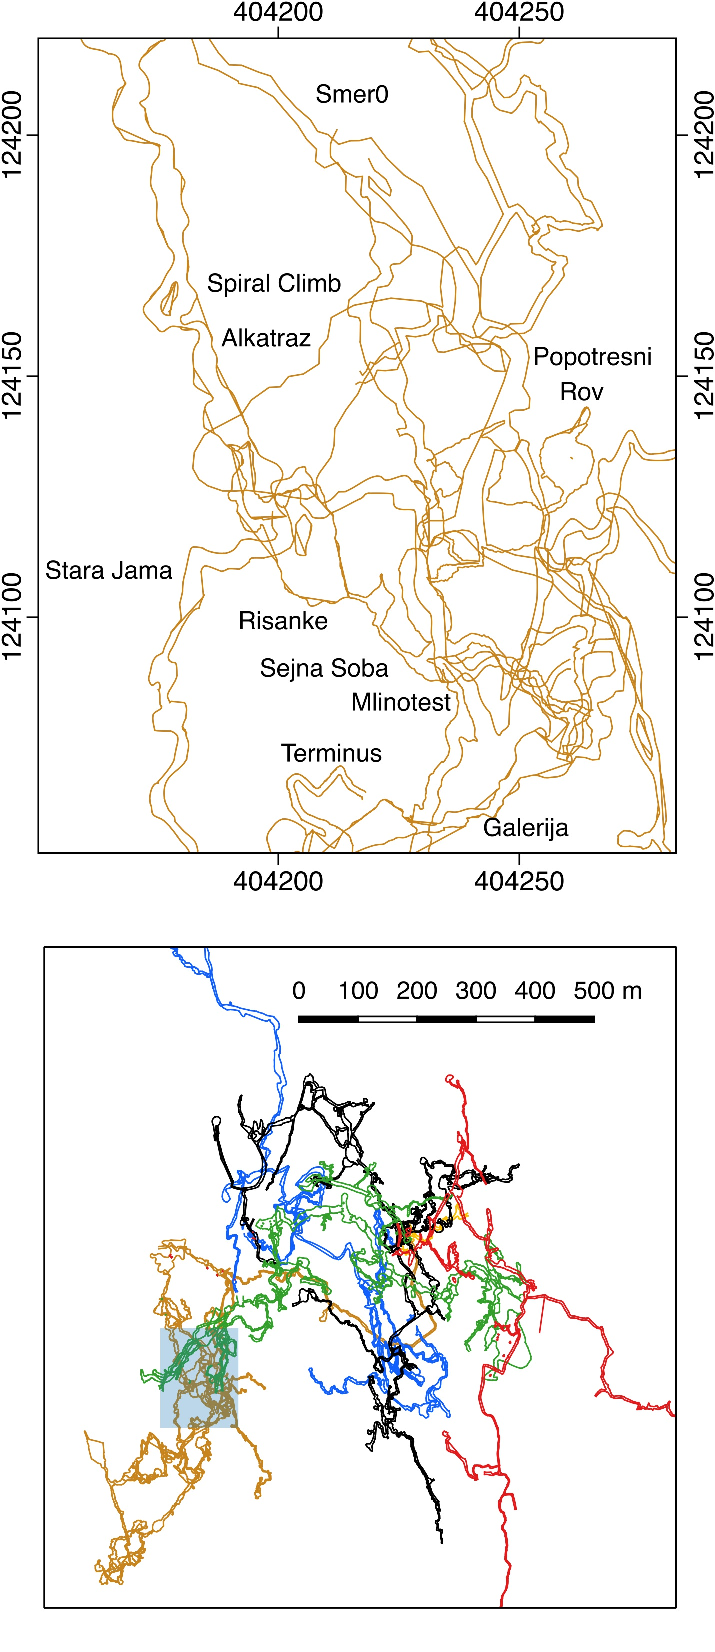
\includegraphics[width=\linewidth]{images/little_insets/alk_inset.pdf}
 \caption{Plan view of the extensions in and around the impressive \protect\passage{Alkatraz} chamber. Slovenian National Grid ESPG 3794}
 \label{Alkatraz inset}
\end{marginfigure}


\margininbox{The Rock}{
		\begin{citemize}
		\item Jack Hare
		\item William Scott
		\end{citemize}}{\explo}
The previous day I'd free climbed up above the \passage{Spiral Climb} and found a squeeze with a big draft and a dark void behind. Keen to do some actual exploration, I convinced Will to go pushing with me. I don't remember having any rope or bolting equipment, so we moved quickly and after pausing a few times to point out to Will how excellent the rigging was now, we got to my lead.

Will didn't seem fazed by the free climbing - it's in an old streamway with plenty of ledges, so never feels that exposed, and so there we were standing and looking up at the squeeze. There was one big boulder wedged in the rift, with a range of smaller ones on the left, but it wasn't a big boulder choke. Will took off his SRT kit and started to wiggle through. He quickly realised his helmet was the limiting factor, so I suggested he took it off. After worryingly little hesitation he did so and grunted his way through.

On the other side the prognosis was good, and given I'd inserted Will into the squeeze it seemed only fair I have a go as well. I only had to do it once, but it was quite tight, but soon I was through and could see we were in a small chamber with one wall missing and a loose, rocky floor. Looking back at the squeeze I could see a big, flat rock that was obviously forming most of the constriction. Will looked nervous and begged me to stop as I pulled and tugged at it, apparently worried that I'd trap us in this chamber forever, but we both agreed that once that rock was gone the squeeze was very straightforwards.

Will stayed in the small chamber to push a lead that quickly died, and \bignote{I went to the missing wall. It opened out into a vast dark space}, with a steep muddy slope down to a floor strewn with massive boulders. We'd done it! We'd found a huge chamber on the first day of pushing! Down at the bottom we conducted a methodical search, checking round all of the walls for leads. Will found a way down to the right of the muddy slope, and went to have a quick looks whilst I kept circling.

\begin{pagefigure}
	\checkoddpage \ifoddpage \forcerectofloat \else \forceversofloat \fi
	\centering
	
   	\begin{subfigure}[t]{0.49\textwidth}
    	\centering
     	\frame{\includegraphics[width=\linewidth]{"images/2016/jack-begin-2016/rhystyers-spiralclimb".jpg}}
       	\caption{} \label{The spiral climb}
    \end{subfigure}
    \hfill
	\begin{subfigure}[t]{0.49\textwidth}
		\centering
		\frame{\includegraphics[width=\linewidth,]{"images/2016/jack-begin-2016/alkatraz".jpg}}
		 \caption{}\label{Alkatraz}
	\end{subfigure}
    \vspace{0cm}
	
	\begin{subfigure}[h]{\textwidth}
		\centering
		\frame{\includegraphics[width=\linewidth,]{"images/2016/jack-begin-2016/will_scott_bolting".jpg}}
		\caption{}\label{WS bolting}
	\end{subfigure}

         \caption{
   		\emph{(a)} The \protect\passage{Spiral Climb} in Primadona where \protect\passage{The Rock} begins
     		\emph{(b)} \protect\passage{Alkatraz} chamber, which can be accessed via \protect\passage[cave]{Monatip} and \protect\passage[cave]{Primadona} via \protect\passage{The Rock}
     		\emph{(c)} Will Scott bolting in the upper levels of \protect\passage[cave]{Primadona} \pic{Rhys Tyers}
		}
\end{pagefigure}

Soon I found a way up on a boulder slope, and quickly got into a streamway. Here my hopes were dashed - a cairn! Someone had been here before. I began to suspect that this was indeed \passage{Alkatraz}, a cavern that I knew was massive but had thought was further away. Back in the main chamber I couldn't find Will, and although I hollered and shouted he didn't respond. This was bad -- I'd lost a fresher already, and the club was having a bad track record this year. After a bit more shouting \bignote{Will emerged, oblivious to the heart ache he'd caused me. Apparently his lead didn't go}, so we checked out the rest of the chamber together, finding a PSS from Tetley in 2000 which confirmed we were in \passage{Alkatraz}.

We checked out Will's lead, and I realised a bit of digging was necessary to get through a crawl with a loose muddy floor filled with small bits of white rock. This happened a few more times as we looped through a series of turns before we popped out at a clean washed aven of dark rock. Free climbing down got us to a streamway which quickly tightened up, but climbing up the other side and over got to an old fossil passage. This was pushed for a bit until we found a small chamber with a chocolate bar wrapper on a cairn. A bit further one we found some more PSS from Tetley, though the numbers and the years were confusing.

Down from this chamber is a big streamway that is reached by downclimbing from ledges. We followed this down stream and into a small wet chamber where the water flows into a crack. Back tracking, we found a big chamber, but lacked the rope to descend. There was a single spit in the wall, badly placed. It's possible this has never been descended, and none of this cave is on the survey

We decided not to survey as we'd heard Tetley had a route from the bottom of \passage{Alkatraz} into other places (again, not on the survey) and returned to the chamber, finding another route out - it's a real maze under \passage{Alkatraz}! We pushed a few more leads, including an unbelievably grim hading rift that ended in me feet first, on my back slowing wriggling down and trying to feel ahead with my feet.

Surveying out, we decided to call our route \passage{The Rock}, as we broke into \passage{Alkatraz}, just like in the best ever Sean Connery film.

\name{Jack Hare}
